\documentclass[twoside]{book}

% Packages required by doxygen
\usepackage{fixltx2e}
\usepackage{calc}
\usepackage{doxygen}
\usepackage[export]{adjustbox} % also loads graphicx
\usepackage{graphicx}
\usepackage[utf8]{inputenc}
\usepackage{makeidx}
\usepackage{multicol}
\usepackage{multirow}
\PassOptionsToPackage{warn}{textcomp}
\usepackage{textcomp}
\usepackage[nointegrals]{wasysym}
\usepackage[table]{xcolor}

% Font selection
\usepackage[T1]{fontenc}
\usepackage[scaled=.90]{helvet}
\usepackage{courier}
\usepackage{amssymb}
\usepackage{sectsty}
\renewcommand{\familydefault}{\sfdefault}
\allsectionsfont{%
  \fontseries{bc}\selectfont%
  \color{darkgray}%
}
\renewcommand{\DoxyLabelFont}{%
  \fontseries{bc}\selectfont%
  \color{darkgray}%
}
\newcommand{\+}{\discretionary{\mbox{\scriptsize$\hookleftarrow$}}{}{}}

% Page & text layout
\usepackage{geometry}
\geometry{%
  a4paper,%
  top=2.5cm,%
  bottom=2.5cm,%
  left=2.5cm,%
  right=2.5cm%
}
\tolerance=750
\hfuzz=15pt
\hbadness=750
\setlength{\emergencystretch}{15pt}
\setlength{\parindent}{0cm}
\setlength{\parskip}{3ex plus 2ex minus 2ex}
\makeatletter
\renewcommand{\paragraph}{%
  \@startsection{paragraph}{4}{0ex}{-1.0ex}{1.0ex}{%
    \normalfont\normalsize\bfseries\SS@parafont%
  }%
}
\renewcommand{\subparagraph}{%
  \@startsection{subparagraph}{5}{0ex}{-1.0ex}{1.0ex}{%
    \normalfont\normalsize\bfseries\SS@subparafont%
  }%
}
\makeatother

% Headers & footers
\usepackage{fancyhdr}
\pagestyle{fancyplain}
\fancyhead[LE]{\fancyplain{}{\bfseries\thepage}}
\fancyhead[CE]{\fancyplain{}{}}
\fancyhead[RE]{\fancyplain{}{\bfseries\leftmark}}
\fancyhead[LO]{\fancyplain{}{\bfseries\rightmark}}
\fancyhead[CO]{\fancyplain{}{}}
\fancyhead[RO]{\fancyplain{}{\bfseries\thepage}}
\fancyfoot[LE]{\fancyplain{}{}}
\fancyfoot[CE]{\fancyplain{}{}}
\fancyfoot[RE]{\fancyplain{}{\bfseries\scriptsize Generated by Doxygen }}
\fancyfoot[LO]{\fancyplain{}{\bfseries\scriptsize Generated by Doxygen }}
\fancyfoot[CO]{\fancyplain{}{}}
\fancyfoot[RO]{\fancyplain{}{}}
\renewcommand{\footrulewidth}{0.4pt}
\renewcommand{\chaptermark}[1]{%
  \markboth{#1}{}%
}
\renewcommand{\sectionmark}[1]{%
  \markright{\thesection\ #1}%
}

% Indices & bibliography
\usepackage{natbib}
\usepackage[titles]{tocloft}
\setcounter{tocdepth}{3}
\setcounter{secnumdepth}{5}
\makeindex

% Hyperlinks (required, but should be loaded last)
\usepackage{ifpdf}
\ifpdf
  \usepackage[pdftex,pagebackref=true]{hyperref}
\else
  \usepackage[ps2pdf,pagebackref=true]{hyperref}
\fi
\hypersetup{%
  colorlinks=true,%
  linkcolor=blue,%
  citecolor=blue,%
  unicode%
}

% Custom commands
\newcommand{\clearemptydoublepage}{%
  \newpage{\pagestyle{empty}\cleardoublepage}%
}

\usepackage{caption}
\captionsetup{labelsep=space,justification=centering,font={bf},singlelinecheck=off,skip=4pt,position=top}

%===== C O N T E N T S =====

\begin{document}

% Titlepage & ToC
\hypersetup{pageanchor=false,
             bookmarksnumbered=true,
             pdfencoding=unicode
            }
\pagenumbering{alph}
\begin{titlepage}
\vspace*{7cm}
\begin{center}%
{\Large C\+M\+S\+C516-\/\+Sem\+Eval2018-\/\+Task6 }\\
\vspace*{1cm}
{\large Generated by Doxygen 1.8.14}\\
\end{center}
\end{titlepage}
\clearemptydoublepage
\pagenumbering{roman}
\tableofcontents
\clearemptydoublepage
\pagenumbering{arabic}
\hypersetup{pageanchor=true}

%--- Begin generated contents ---
\chapter{C\+M\+S\+C516}
\label{md_README}
\Hypertarget{md_README}
\input{md_README}
\chapter{Namespace Index}
\section{Namespace List}
Here is a list of all namespaces with brief descriptions\+:\begin{DoxyCompactList}
\item\contentsline{section}{\hyperlink{namespacesetup}{setup} }{\pageref{namespacesetup}}{}
\item\contentsline{section}{\hyperlink{namespacetask6}{task6} }{\pageref{namespacetask6}}{}
\item\contentsline{section}{\hyperlink{namespacetask6_1_1sutime}{task6.\+sutime} }{\pageref{namespacetask6_1_1sutime}}{}
\item\contentsline{section}{\hyperlink{namespacetask6_1_1sutime__wrapper}{task6.\+sutime\+\_\+wrapper} }{\pageref{namespacetask6_1_1sutime__wrapper}}{}
\item\contentsline{section}{\hyperlink{namespacetask6_1_1t6Entities}{task6.\+t6\+Entities} }{\pageref{namespacetask6_1_1t6Entities}}{}
\item\contentsline{section}{\hyperlink{namespacetask6_1_1utils}{task6.\+utils} }{\pageref{namespacetask6_1_1utils}}{}
\item\contentsline{section}{\hyperlink{namespacetest}{test} }{\pageref{namespacetest}}{}
\item\contentsline{section}{\hyperlink{namespacetest_1_1test}{test.\+test} }{\pageref{namespacetest_1_1test}}{}
\end{DoxyCompactList}

\chapter{Hierarchical Index}
\section{Class Hierarchy}
This inheritance list is sorted roughly, but not completely, alphabetically\+:\begin{DoxyCompactList}
\item object\begin{DoxyCompactList}
\item \contentsline{section}{task6.\+sutime.\+S\+U\+Time}{\pageref{classtask6_1_1sutime_1_1SUTime}}{}
\end{DoxyCompactList}
\item \contentsline{section}{task6.\+t6\+Entities.\+t6\+Entity}{\pageref{classtask6_1_1t6Entities_1_1t6Entity}}{}
\begin{DoxyCompactList}
\item \contentsline{section}{task6.\+t6\+Entities.\+t6\+Interval\+Entity}{\pageref{classtask6_1_1t6Entities_1_1t6IntervalEntity}}{}
\item \contentsline{section}{task6.\+t6\+Entities.\+t6\+Operator}{\pageref{classtask6_1_1t6Entities_1_1t6Operator}}{}
\item \contentsline{section}{task6.\+t6\+Entities.\+t6\+Period\+Entity}{\pageref{classtask6_1_1t6Entities_1_1t6PeriodEntity}}{}
\item \contentsline{section}{task6.\+t6\+Entities.\+t6\+Repeating\+Interval\+Entity}{\pageref{classtask6_1_1t6Entities_1_1t6RepeatingIntervalEntity}}{}
\end{DoxyCompactList}
\end{DoxyCompactList}

\chapter{Class Index}
\section{Class List}
Here are the classes, structs, unions and interfaces with brief descriptions\+:\begin{DoxyCompactList}
\item\contentsline{section}{\hyperlink{classtask6_1_1sutime_1_1SUTime}{task6.\+sutime.\+S\+U\+Time} }{\pageref{classtask6_1_1sutime_1_1SUTime}}{}
\item\contentsline{section}{\hyperlink{classtask6_1_1t6Entities_1_1T6AfterOperator}{task6.\+t6\+Entities.\+T6\+After\+Operator} }{\pageref{classtask6_1_1t6Entities_1_1T6AfterOperator}}{}
\item\contentsline{section}{\hyperlink{classtask6_1_1t6Entities_1_1T6AMPMOfDay}{task6.\+t6\+Entities.\+T6\+A\+M\+P\+M\+Of\+Day} }{\pageref{classtask6_1_1t6Entities_1_1T6AMPMOfDay}}{}
\item\contentsline{section}{\hyperlink{classtask6_1_1t6Entities_1_1T6BeforeOperator}{task6.\+t6\+Entities.\+T6\+Before\+Operator} }{\pageref{classtask6_1_1t6Entities_1_1T6BeforeOperator}}{}
\item\contentsline{section}{\hyperlink{classtask6_1_1t6Entities_1_1T6BetweenOperator}{task6.\+t6\+Entities.\+T6\+Between\+Operator} }{\pageref{classtask6_1_1t6Entities_1_1T6BetweenOperator}}{}
\item\contentsline{section}{\hyperlink{classtask6_1_1t6Entities_1_1T6CalendarIntervalEntity}{task6.\+t6\+Entities.\+T6\+Calendar\+Interval\+Entity} }{\pageref{classtask6_1_1t6Entities_1_1T6CalendarIntervalEntity}}{}
\item\contentsline{section}{\hyperlink{classtask6_1_1t6Entities_1_1T6DayOfMonthEntity}{task6.\+t6\+Entities.\+T6\+Day\+Of\+Month\+Entity} }{\pageref{classtask6_1_1t6Entities_1_1T6DayOfMonthEntity}}{}
\item\contentsline{section}{\hyperlink{classtask6_1_1t6Entities_1_1T6DayOfWeekEntity}{task6.\+t6\+Entities.\+T6\+Day\+Of\+Week\+Entity} }{\pageref{classtask6_1_1t6Entities_1_1T6DayOfWeekEntity}}{}
\item\contentsline{section}{\hyperlink{classtask6_1_1t6Entities_1_1T6DifferenceOperator}{task6.\+t6\+Entities.\+T6\+Difference\+Operator} }{\pageref{classtask6_1_1t6Entities_1_1T6DifferenceOperator}}{}
\item\contentsline{section}{\hyperlink{classtask6_1_1t6Entities_1_1T6Entity}{task6.\+t6\+Entities.\+T6\+Entity} \\*Class definitions for all Time\+Norm entities -\/ Intervals, Periods, Repeating-\/\+Intervals, and Operators }{\pageref{classtask6_1_1t6Entities_1_1T6Entity}}{}
\item\contentsline{section}{\hyperlink{classtask6_1_1t6Entities_1_1T6Event}{task6.\+t6\+Entities.\+T6\+Event} }{\pageref{classtask6_1_1t6Entities_1_1T6Event}}{}
\item\contentsline{section}{\hyperlink{classtask6_1_1t6Entities_1_1T6EveryNthOperator}{task6.\+t6\+Entities.\+T6\+Every\+Nth\+Operator} }{\pageref{classtask6_1_1t6Entities_1_1T6EveryNthOperator}}{}
\item\contentsline{section}{\hyperlink{classtask6_1_1t6Entities_1_1T6HourOfDayEntity}{task6.\+t6\+Entities.\+T6\+Hour\+Of\+Day\+Entity} }{\pageref{classtask6_1_1t6Entities_1_1T6HourOfDayEntity}}{}
\item\contentsline{section}{\hyperlink{classtask6_1_1t6Entities_1_1T6IntersectionOperator}{task6.\+t6\+Entities.\+T6\+Intersection\+Operator} }{\pageref{classtask6_1_1t6Entities_1_1T6IntersectionOperator}}{}
\item\contentsline{section}{\hyperlink{classtask6_1_1t6Entities_1_1T6IntervalEntity}{task6.\+t6\+Entities.\+T6\+Interval\+Entity} \\*An interval, just super classes for year interval for consistency }{\pageref{classtask6_1_1t6Entities_1_1T6IntervalEntity}}{}
\item\contentsline{section}{\hyperlink{classtask6_1_1t6Entities_1_1T6LastOperator}{task6.\+t6\+Entities.\+T6\+Last\+Operator} \\*Create a last(\+Period) or last(Repeating-\/\+Interval) operator }{\pageref{classtask6_1_1t6Entities_1_1T6LastOperator}}{}
\item\contentsline{section}{\hyperlink{classtask6_1_1t6Entities_1_1T6MinuteOfHourEntity}{task6.\+t6\+Entities.\+T6\+Minute\+Of\+Hour\+Entity} }{\pageref{classtask6_1_1t6Entities_1_1T6MinuteOfHourEntity}}{}
\item\contentsline{section}{\hyperlink{classtask6_1_1t6Entities_1_1T6Modifier}{task6.\+t6\+Entities.\+T6\+Modifier} }{\pageref{classtask6_1_1t6Entities_1_1T6Modifier}}{}
\item\contentsline{section}{\hyperlink{classtask6_1_1t6Entities_1_1T6MonthOfYearEntity}{task6.\+t6\+Entities.\+T6\+Month\+Of\+Year\+Entity} }{\pageref{classtask6_1_1t6Entities_1_1T6MonthOfYearEntity}}{}
\item\contentsline{section}{\hyperlink{classtask6_1_1t6Entities_1_1T6NextOperator}{task6.\+t6\+Entities.\+T6\+Next\+Operator} }{\pageref{classtask6_1_1t6Entities_1_1T6NextOperator}}{}
\item\contentsline{section}{\hyperlink{classtask6_1_1t6Entities_1_1T6NthOperator}{task6.\+t6\+Entities.\+T6\+Nth\+Operator} }{\pageref{classtask6_1_1t6Entities_1_1T6NthOperator}}{}
\item\contentsline{section}{\hyperlink{classtask6_1_1t6Entities_1_1T6Number}{task6.\+t6\+Entities.\+T6\+Number} }{\pageref{classtask6_1_1t6Entities_1_1T6Number}}{}
\item\contentsline{section}{\hyperlink{classtask6_1_1t6Entities_1_1T6Operator}{task6.\+t6\+Entities.\+T6\+Operator} }{\pageref{classtask6_1_1t6Entities_1_1T6Operator}}{}
\item\contentsline{section}{\hyperlink{classtask6_1_1t6Entities_1_1T6PartOfDayEntity}{task6.\+t6\+Entities.\+T6\+Part\+Of\+Day\+Entity} }{\pageref{classtask6_1_1t6Entities_1_1T6PartOfDayEntity}}{}
\item\contentsline{section}{\hyperlink{classtask6_1_1t6Entities_1_1T6PeriodEntity}{task6.\+t6\+Entities.\+T6\+Period\+Entity} }{\pageref{classtask6_1_1t6Entities_1_1T6PeriodEntity}}{}
\item\contentsline{section}{\hyperlink{classtask6_1_1t6Entities_1_1T6repeatingIntervalEntity}{task6.\+t6\+Entities.\+T6repeating\+Interval\+Entity} }{\pageref{classtask6_1_1t6Entities_1_1T6repeatingIntervalEntity}}{}
\item\contentsline{section}{\hyperlink{classtask6_1_1t6Entities_1_1T6SecondOfMinuteEntity}{task6.\+t6\+Entities.\+T6\+Second\+Of\+Minute\+Entity} }{\pageref{classtask6_1_1t6Entities_1_1T6SecondOfMinuteEntity}}{}
\item\contentsline{section}{\hyperlink{classtask6_1_1t6Entities_1_1T6SumOperator}{task6.\+t6\+Entities.\+T6\+Sum\+Operator} }{\pageref{classtask6_1_1t6Entities_1_1T6SumOperator}}{}
\item\contentsline{section}{\hyperlink{classtask6_1_1t6Entities_1_1T6ThisOperator}{task6.\+t6\+Entities.\+T6\+This\+Operator} }{\pageref{classtask6_1_1t6Entities_1_1T6ThisOperator}}{}
\item\contentsline{section}{\hyperlink{classtask6_1_1t6Entities_1_1T6time__zoneEntity}{task6.\+t6\+Entities.\+T6time\+\_\+zone\+Entity} }{\pageref{classtask6_1_1t6Entities_1_1T6time__zoneEntity}}{}
\item\contentsline{section}{\hyperlink{classtask6_1_1t6Entities_1_1T6TwoDigitYearOperator}{task6.\+t6\+Entities.\+T6\+Two\+Digit\+Year\+Operator} }{\pageref{classtask6_1_1t6Entities_1_1T6TwoDigitYearOperator}}{}
\item\contentsline{section}{\hyperlink{classtask6_1_1t6Entities_1_1T6UnionOperator}{task6.\+t6\+Entities.\+T6\+Union\+Operator} }{\pageref{classtask6_1_1t6Entities_1_1T6UnionOperator}}{}
\item\contentsline{section}{\hyperlink{classtask6_1_1t6Entities_1_1T6WeekOfYearEntity}{task6.\+t6\+Entities.\+T6\+Week\+Of\+Year\+Entity} }{\pageref{classtask6_1_1t6Entities_1_1T6WeekOfYearEntity}}{}
\item\contentsline{section}{\hyperlink{classtask6_1_1t6Entities_1_1T6YearEntity}{task6.\+t6\+Entities.\+T6\+Year\+Entity} \\*A year interval }{\pageref{classtask6_1_1t6Entities_1_1T6YearEntity}}{}
\end{DoxyCompactList}

\chapter{File Index}
\section{File List}
Here is a list of all files with brief descriptions\+:\begin{DoxyCompactList}
\item\contentsline{section}{\hyperlink{setup_8py}{setup.\+py} }{\pageref{setup_8py}}{}
\item\contentsline{section}{\hyperlink{test_8py}{test.\+py} }{\pageref{test_8py}}{}
\item\contentsline{section}{task6/\hyperlink{task6_2____init_____8py}{\+\_\+\+\_\+init\+\_\+\+\_\+.\+py} }{\pageref{task6_2____init_____8py}}{}
\item\contentsline{section}{task6/\hyperlink{sutime_8py}{sutime.\+py} }{\pageref{sutime_8py}}{}
\item\contentsline{section}{task6/\hyperlink{sutime__wrapper_8py}{sutime\+\_\+wrapper.\+py} }{\pageref{sutime__wrapper_8py}}{}
\item\contentsline{section}{task6/\hyperlink{t6Entities_8py}{t6\+Entities.\+py} }{\pageref{t6Entities_8py}}{}
\item\contentsline{section}{task6/\hyperlink{utils_8py}{utils.\+py} }{\pageref{utils_8py}}{}
\item\contentsline{section}{test/\hyperlink{test_2____init_____8py}{\+\_\+\+\_\+init\+\_\+\+\_\+.\+py} }{\pageref{test_2____init_____8py}}{}
\item\contentsline{section}{test/\hyperlink{test_2test_8py}{test.\+py} }{\pageref{test_2test_8py}}{}
\end{DoxyCompactList}

\chapter{Namespace Documentation}
\hypertarget{namespacesetup}{}\section{setup Namespace Reference}
\label{namespacesetup}\index{setup@{setup}}
\subsection*{Variables}
\begin{DoxyCompactItemize}
\item 
\hyperlink{namespacesetup_a9c076537d899ffd8096e58c282bb7b02}{here} = path.\+abspath(path.\+dirname(\+\_\+\+\_\+file\+\_\+\+\_\+))
\item 
\hyperlink{namespacesetup_a443be2d01fd539bf6761aff70724d876}{encoding}
\item 
\hyperlink{namespacesetup_a4cda9dbfb952875376a0749fe08a5bde}{long\+\_\+description} = f.\+read()
\item 
\hyperlink{namespacesetup_ab3a7a0638d76a01367c5bc3cc699447f}{name}
\item 
\hyperlink{namespacesetup_a2aa722b36a933088812b50ea79b97a5c}{version}
\item 
\hyperlink{namespacesetup_aedf461ec52a946bda975938ba0b93ec0}{description}
\item 
\hyperlink{namespacesetup_afc13124aa5c0124e84e1d965e3f4b0fb}{url}
\item 
\hyperlink{namespacesetup_a3a57a4772d418a06835249cbade0d86a}{author}
\item 
\hyperlink{namespacesetup_a5b08034343aa2be607722a8b315f3625}{author\+\_\+email}
\item 
\hyperlink{namespacesetup_a8ed6f50a28bd6a8794f8e1153baa6de9}{license}
\item 
\hyperlink{namespacesetup_abe96a9c38c1c61f9f0fdb002c482f785}{classifiers}
\item 
\hyperlink{namespacesetup_a73ae9ecb109f0dcab6f0b6a89043c5c3}{keywords}
\item 
\hyperlink{namespacesetup_aff2375a361fd5865c77bd9aa093be747}{packages}
\item 
\hyperlink{namespacesetup_abead4f26b530856f858f0d44c7cf2588}{install\+\_\+requires}
\end{DoxyCompactItemize}


\subsection{Variable Documentation}
\mbox{\Hypertarget{namespacesetup_a3a57a4772d418a06835249cbade0d86a}\label{namespacesetup_a3a57a4772d418a06835249cbade0d86a}} 
\index{setup@{setup}!author@{author}}
\index{author@{author}!setup@{setup}}
\subsubsection{\texorpdfstring{author}{author}}
{\footnotesize\ttfamily setup.\+author}

\mbox{\Hypertarget{namespacesetup_a5b08034343aa2be607722a8b315f3625}\label{namespacesetup_a5b08034343aa2be607722a8b315f3625}} 
\index{setup@{setup}!author\+\_\+email@{author\+\_\+email}}
\index{author\+\_\+email@{author\+\_\+email}!setup@{setup}}
\subsubsection{\texorpdfstring{author\+\_\+email}{author\_email}}
{\footnotesize\ttfamily setup.\+author\+\_\+email}

\mbox{\Hypertarget{namespacesetup_abe96a9c38c1c61f9f0fdb002c482f785}\label{namespacesetup_abe96a9c38c1c61f9f0fdb002c482f785}} 
\index{setup@{setup}!classifiers@{classifiers}}
\index{classifiers@{classifiers}!setup@{setup}}
\subsubsection{\texorpdfstring{classifiers}{classifiers}}
{\footnotesize\ttfamily setup.\+classifiers}

\mbox{\Hypertarget{namespacesetup_aedf461ec52a946bda975938ba0b93ec0}\label{namespacesetup_aedf461ec52a946bda975938ba0b93ec0}} 
\index{setup@{setup}!description@{description}}
\index{description@{description}!setup@{setup}}
\subsubsection{\texorpdfstring{description}{description}}
{\footnotesize\ttfamily setup.\+description}

\mbox{\Hypertarget{namespacesetup_a443be2d01fd539bf6761aff70724d876}\label{namespacesetup_a443be2d01fd539bf6761aff70724d876}} 
\index{setup@{setup}!encoding@{encoding}}
\index{encoding@{encoding}!setup@{setup}}
\subsubsection{\texorpdfstring{encoding}{encoding}}
{\footnotesize\ttfamily setup.\+encoding}

\mbox{\Hypertarget{namespacesetup_a9c076537d899ffd8096e58c282bb7b02}\label{namespacesetup_a9c076537d899ffd8096e58c282bb7b02}} 
\index{setup@{setup}!here@{here}}
\index{here@{here}!setup@{setup}}
\subsubsection{\texorpdfstring{here}{here}}
{\footnotesize\ttfamily setup.\+here = path.\+abspath(path.\+dirname(\+\_\+\+\_\+file\+\_\+\+\_\+))}

\mbox{\Hypertarget{namespacesetup_abead4f26b530856f858f0d44c7cf2588}\label{namespacesetup_abead4f26b530856f858f0d44c7cf2588}} 
\index{setup@{setup}!install\+\_\+requires@{install\+\_\+requires}}
\index{install\+\_\+requires@{install\+\_\+requires}!setup@{setup}}
\subsubsection{\texorpdfstring{install\+\_\+requires}{install\_requires}}
{\footnotesize\ttfamily setup.\+install\+\_\+requires}

\mbox{\Hypertarget{namespacesetup_a73ae9ecb109f0dcab6f0b6a89043c5c3}\label{namespacesetup_a73ae9ecb109f0dcab6f0b6a89043c5c3}} 
\index{setup@{setup}!keywords@{keywords}}
\index{keywords@{keywords}!setup@{setup}}
\subsubsection{\texorpdfstring{keywords}{keywords}}
{\footnotesize\ttfamily setup.\+keywords}

\mbox{\Hypertarget{namespacesetup_a8ed6f50a28bd6a8794f8e1153baa6de9}\label{namespacesetup_a8ed6f50a28bd6a8794f8e1153baa6de9}} 
\index{setup@{setup}!license@{license}}
\index{license@{license}!setup@{setup}}
\subsubsection{\texorpdfstring{license}{license}}
{\footnotesize\ttfamily setup.\+license}

\mbox{\Hypertarget{namespacesetup_a4cda9dbfb952875376a0749fe08a5bde}\label{namespacesetup_a4cda9dbfb952875376a0749fe08a5bde}} 
\index{setup@{setup}!long\+\_\+description@{long\+\_\+description}}
\index{long\+\_\+description@{long\+\_\+description}!setup@{setup}}
\subsubsection{\texorpdfstring{long\+\_\+description}{long\_description}}
{\footnotesize\ttfamily setup.\+long\+\_\+description = f.\+read()}

\mbox{\Hypertarget{namespacesetup_ab3a7a0638d76a01367c5bc3cc699447f}\label{namespacesetup_ab3a7a0638d76a01367c5bc3cc699447f}} 
\index{setup@{setup}!name@{name}}
\index{name@{name}!setup@{setup}}
\subsubsection{\texorpdfstring{name}{name}}
{\footnotesize\ttfamily setup.\+name}

\mbox{\Hypertarget{namespacesetup_aff2375a361fd5865c77bd9aa093be747}\label{namespacesetup_aff2375a361fd5865c77bd9aa093be747}} 
\index{setup@{setup}!packages@{packages}}
\index{packages@{packages}!setup@{setup}}
\subsubsection{\texorpdfstring{packages}{packages}}
{\footnotesize\ttfamily setup.\+packages}

\mbox{\Hypertarget{namespacesetup_afc13124aa5c0124e84e1d965e3f4b0fb}\label{namespacesetup_afc13124aa5c0124e84e1d965e3f4b0fb}} 
\index{setup@{setup}!url@{url}}
\index{url@{url}!setup@{setup}}
\subsubsection{\texorpdfstring{url}{url}}
{\footnotesize\ttfamily setup.\+url}

\mbox{\Hypertarget{namespacesetup_a2aa722b36a933088812b50ea79b97a5c}\label{namespacesetup_a2aa722b36a933088812b50ea79b97a5c}} 
\index{setup@{setup}!version@{version}}
\index{version@{version}!setup@{setup}}
\subsubsection{\texorpdfstring{version}{version}}
{\footnotesize\ttfamily setup.\+version}


\hypertarget{namespacetask6}{}\section{task6 Namespace Reference}
\label{namespacetask6}\index{task6@{task6}}
\subsection*{Namespaces}
\begin{DoxyCompactItemize}
\item 
 \hyperlink{namespacetask6_1_1sutime}{sutime}
\item 
 \hyperlink{namespacetask6_1_1sutime__wrapper}{sutime\+\_\+wrapper}
\item 
 \hyperlink{namespacetask6_1_1t6Entities}{t6\+Entities}
\item 
 \hyperlink{namespacetask6_1_1utils}{utils}
\end{DoxyCompactItemize}

\hypertarget{namespacetask6_1_1sutime}{}\section{task6.\+sutime Namespace Reference}
\label{namespacetask6_1_1sutime}\index{task6.\+sutime@{task6.\+sutime}}
\subsection*{Classes}
\begin{DoxyCompactItemize}
\item 
class \hyperlink{classtask6_1_1sutime_1_1SUTime}{S\+U\+Time}
\end{DoxyCompactItemize}

\hypertarget{namespacetask6_1_1sutime__wrapper}{}\section{task6.\+sutime\+\_\+wrapper Namespace Reference}
\label{namespacetask6_1_1sutime__wrapper}\index{task6.\+sutime\+\_\+wrapper@{task6.\+sutime\+\_\+wrapper}}
\subsection*{Functions}
\begin{DoxyCompactItemize}
\item 
def \hyperlink{namespacetask6_1_1sutime__wrapper_af4cac751d594757efbe539a28850ff28}{call\+S\+U\+Time\+Parse} (file\+\_\+path)
\begin{DoxyCompactList}\small\item\em call\+S\+U\+T\+I\+M\+E\+Parse() Function Purpose\+: Takes in raw text file and performs S\+U\+Time\textquotesingle{}s algorithm on \#it and returns it in J\+S\+ON format. \end{DoxyCompactList}\end{DoxyCompactItemize}


\subsection{Function Documentation}
\mbox{\Hypertarget{namespacetask6_1_1sutime__wrapper_af4cac751d594757efbe539a28850ff28}\label{namespacetask6_1_1sutime__wrapper_af4cac751d594757efbe539a28850ff28}} 
\index{task6\+::sutime\+\_\+wrapper@{task6\+::sutime\+\_\+wrapper}!call\+S\+U\+Time\+Parse@{call\+S\+U\+Time\+Parse}}
\index{call\+S\+U\+Time\+Parse@{call\+S\+U\+Time\+Parse}!task6\+::sutime\+\_\+wrapper@{task6\+::sutime\+\_\+wrapper}}
\subsubsection{\texorpdfstring{call\+S\+U\+Time\+Parse()}{callSUTimeParse()}}
{\footnotesize\ttfamily def task6.\+sutime\+\_\+wrapper.\+call\+S\+U\+Time\+Parse (\begin{DoxyParamCaption}\item[{}]{file\+\_\+path }\end{DoxyParamCaption})}



call\+S\+U\+T\+I\+M\+E\+Parse() Function Purpose\+: Takes in raw text file and performs S\+U\+Time\textquotesingle{}s algorithm on \#it and returns it in J\+S\+ON format. 

Input\+: String containing the location and name of the text file to be parsed. Output\+: J\+S\+ON string output of raw input file 
\hypertarget{namespacetask6_1_1t6Entities}{}\section{task6.\+t6\+Entities Namespace Reference}
\label{namespacetask6_1_1t6Entities}\index{task6.\+t6\+Entities@{task6.\+t6\+Entities}}
\subsection*{Classes}
\begin{DoxyCompactItemize}
\item 
class \hyperlink{classtask6_1_1t6Entities_1_1T6AfterOperator}{T6\+After\+Operator}
\item 
class \hyperlink{classtask6_1_1t6Entities_1_1T6AMPMOfDay}{T6\+A\+M\+P\+M\+Of\+Day}
\item 
class \hyperlink{classtask6_1_1t6Entities_1_1T6BeforeOperator}{T6\+Before\+Operator}
\item 
class \hyperlink{classtask6_1_1t6Entities_1_1T6BetweenOperator}{T6\+Between\+Operator}
\item 
class \hyperlink{classtask6_1_1t6Entities_1_1T6CalendarIntervalEntity}{T6\+Calendar\+Interval\+Entity}
\item 
class \hyperlink{classtask6_1_1t6Entities_1_1T6DayOfMonthEntity}{T6\+Day\+Of\+Month\+Entity}
\item 
class \hyperlink{classtask6_1_1t6Entities_1_1T6DayOfWeekEntity}{T6\+Day\+Of\+Week\+Entity}
\item 
class \hyperlink{classtask6_1_1t6Entities_1_1T6DifferenceOperator}{T6\+Difference\+Operator}
\item 
class \hyperlink{classtask6_1_1t6Entities_1_1T6Entity}{T6\+Entity}
\begin{DoxyCompactList}\small\item\em Class definitions for all Time\+Norm entities -\/ Intervals, Periods, Repeating-\/\+Intervals, and Operators. \end{DoxyCompactList}\item 
class \hyperlink{classtask6_1_1t6Entities_1_1T6Event}{T6\+Event}
\item 
class \hyperlink{classtask6_1_1t6Entities_1_1T6EveryNthOperator}{T6\+Every\+Nth\+Operator}
\item 
class \hyperlink{classtask6_1_1t6Entities_1_1T6HourOfDayEntity}{T6\+Hour\+Of\+Day\+Entity}
\item 
class \hyperlink{classtask6_1_1t6Entities_1_1T6IntersectionOperator}{T6\+Intersection\+Operator}
\item 
class \hyperlink{classtask6_1_1t6Entities_1_1T6IntervalEntity}{T6\+Interval\+Entity}
\begin{DoxyCompactList}\small\item\em An interval, just super classes for year interval for consistency. \end{DoxyCompactList}\item 
class \hyperlink{classtask6_1_1t6Entities_1_1T6LastOperator}{T6\+Last\+Operator}
\begin{DoxyCompactList}\small\item\em Create a last(\+Period) or last(Repeating-\/\+Interval) operator. \end{DoxyCompactList}\item 
class \hyperlink{classtask6_1_1t6Entities_1_1T6MinuteOfHourEntity}{T6\+Minute\+Of\+Hour\+Entity}
\item 
class \hyperlink{classtask6_1_1t6Entities_1_1T6Modifier}{T6\+Modifier}
\item 
class \hyperlink{classtask6_1_1t6Entities_1_1T6MonthOfYearEntity}{T6\+Month\+Of\+Year\+Entity}
\item 
class \hyperlink{classtask6_1_1t6Entities_1_1T6NextOperator}{T6\+Next\+Operator}
\item 
class \hyperlink{classtask6_1_1t6Entities_1_1T6NthOperator}{T6\+Nth\+Operator}
\item 
class \hyperlink{classtask6_1_1t6Entities_1_1T6Number}{T6\+Number}
\item 
class \hyperlink{classtask6_1_1t6Entities_1_1T6Operator}{T6\+Operator}
\item 
class \hyperlink{classtask6_1_1t6Entities_1_1T6PartOfDayEntity}{T6\+Part\+Of\+Day\+Entity}
\item 
class \hyperlink{classtask6_1_1t6Entities_1_1T6PeriodEntity}{T6\+Period\+Entity}
\item 
class \hyperlink{classtask6_1_1t6Entities_1_1T6repeatingIntervalEntity}{T6repeating\+Interval\+Entity}
\item 
class \hyperlink{classtask6_1_1t6Entities_1_1T6SecondOfMinuteEntity}{T6\+Second\+Of\+Minute\+Entity}
\item 
class \hyperlink{classtask6_1_1t6Entities_1_1T6SumOperator}{T6\+Sum\+Operator}
\item 
class \hyperlink{classtask6_1_1t6Entities_1_1T6ThisOperator}{T6\+This\+Operator}
\item 
class \hyperlink{classtask6_1_1t6Entities_1_1T6time__zoneEntity}{T6time\+\_\+zone\+Entity}
\item 
class \hyperlink{classtask6_1_1t6Entities_1_1T6TwoDigitYearOperator}{T6\+Two\+Digit\+Year\+Operator}
\item 
class \hyperlink{classtask6_1_1t6Entities_1_1T6UnionOperator}{T6\+Union\+Operator}
\item 
class \hyperlink{classtask6_1_1t6Entities_1_1T6WeekOfYearEntity}{T6\+Week\+Of\+Year\+Entity}
\item 
class \hyperlink{classtask6_1_1t6Entities_1_1T6YearEntity}{T6\+Year\+Entity}
\begin{DoxyCompactList}\small\item\em A year interval. \end{DoxyCompactList}\end{DoxyCompactItemize}

\hypertarget{namespacetask6_1_1utils}{}\section{task6.\+utils Namespace Reference}
\label{namespacetask6_1_1utils}\index{task6.\+utils@{task6.\+utils}}
\subsection*{Functions}
\begin{DoxyCompactItemize}
\item 
def \hyperlink{namespacetask6_1_1utils_a515e86e4cb66853a491562c4dd7935b1}{get\+Whitespace\+Spans} (file\+\_\+path)
\begin{DoxyCompactList}\small\item\em \hyperlink{namespacetask6_1_1utils_a515e86e4cb66853a491562c4dd7935b1}{get\+Whitespace\+Spans()} Function Purpose\+: Pasrses a text file to idenitfy all tokens seperated by white space with their original file span coordinates. \end{DoxyCompactList}\end{DoxyCompactItemize}


\subsection{Function Documentation}
\mbox{\Hypertarget{namespacetask6_1_1utils_a515e86e4cb66853a491562c4dd7935b1}\label{namespacetask6_1_1utils_a515e86e4cb66853a491562c4dd7935b1}} 
\index{task6\+::utils@{task6\+::utils}!get\+Whitespace\+Spans@{get\+Whitespace\+Spans}}
\index{get\+Whitespace\+Spans@{get\+Whitespace\+Spans}!task6\+::utils@{task6\+::utils}}
\subsubsection{\texorpdfstring{get\+Whitespace\+Spans()}{getWhitespaceSpans()}}
{\footnotesize\ttfamily def task6.\+utils.\+get\+Whitespace\+Spans (\begin{DoxyParamCaption}\item[{}]{file\+\_\+path }\end{DoxyParamCaption})}



\hyperlink{namespacetask6_1_1utils_a515e86e4cb66853a491562c4dd7935b1}{get\+Whitespace\+Spans()} Function Purpose\+: Pasrses a text file to idenitfy all tokens seperated by white space with their original file span coordinates. 

Input\+: String containing the location and name of the text file to be parsed. Outputs\+: text -\/ String containing the raw text blob from reading in the file. tokenized\+\_\+text -\/ a list containing each token that was seperated by white space. spans -\/ the coordinates for each token. 

Definition at line 18 of file utils.\+py.


\hypertarget{namespacetest}{}\section{test Namespace Reference}
\label{namespacetest}\index{test@{test}}
\subsection*{Namespaces}
\begin{DoxyCompactItemize}
\item 
 \hyperlink{namespacetest_1_1test}{test}
\end{DoxyCompactItemize}
\subsection*{Variables}
\begin{DoxyCompactItemize}
\item 
\hyperlink{namespacetest_ac1f92ca15306aee561188e0f37aabc66}{r}
\item 
\hyperlink{namespacetest_ae9ebdaf735944736b55d720cfe9c3e02}{t}
\item 
\hyperlink{namespacetest_a91a88df52e09e64ff8cc9e5d8277c8d4}{s}
\end{DoxyCompactItemize}


\subsection{Variable Documentation}
\mbox{\Hypertarget{namespacetest_ac1f92ca15306aee561188e0f37aabc66}\label{namespacetest_ac1f92ca15306aee561188e0f37aabc66}} 
\index{test@{test}!r@{r}}
\index{r@{r}!test@{test}}
\subsubsection{\texorpdfstring{r}{r}}
{\footnotesize\ttfamily test.\+r}

\mbox{\Hypertarget{namespacetest_a91a88df52e09e64ff8cc9e5d8277c8d4}\label{namespacetest_a91a88df52e09e64ff8cc9e5d8277c8d4}} 
\index{test@{test}!s@{s}}
\index{s@{s}!test@{test}}
\subsubsection{\texorpdfstring{s}{s}}
{\footnotesize\ttfamily test.\+s}

\mbox{\Hypertarget{namespacetest_ae9ebdaf735944736b55d720cfe9c3e02}\label{namespacetest_ae9ebdaf735944736b55d720cfe9c3e02}} 
\index{test@{test}!t@{t}}
\index{t@{t}!test@{test}}
\subsubsection{\texorpdfstring{t}{t}}
{\footnotesize\ttfamily test.\+t}


\hypertarget{namespacetest_1_1test}{}\section{test.\+test Namespace Reference}
\label{namespacetest_1_1test}\index{test.\+test@{test.\+test}}
\subsection*{Variables}
\begin{DoxyCompactItemize}
\item 
\hyperlink{namespacetest_1_1test_ac6940ca06224277c08c299101b3296b4}{r}
\item 
\hyperlink{namespacetest_1_1test_a85ce85cce39e2fad621db9c70186235a}{t}
\item 
\hyperlink{namespacetest_1_1test_a4e3f76bc561357031de5269619280f91}{s}
\end{DoxyCompactItemize}


\subsection{Variable Documentation}
\mbox{\Hypertarget{namespacetest_1_1test_ac6940ca06224277c08c299101b3296b4}\label{namespacetest_1_1test_ac6940ca06224277c08c299101b3296b4}} 
\index{test\+::test@{test\+::test}!r@{r}}
\index{r@{r}!test\+::test@{test\+::test}}
\subsubsection{\texorpdfstring{r}{r}}
{\footnotesize\ttfamily test.\+test.\+r}

\mbox{\Hypertarget{namespacetest_1_1test_a4e3f76bc561357031de5269619280f91}\label{namespacetest_1_1test_a4e3f76bc561357031de5269619280f91}} 
\index{test\+::test@{test\+::test}!s@{s}}
\index{s@{s}!test\+::test@{test\+::test}}
\subsubsection{\texorpdfstring{s}{s}}
{\footnotesize\ttfamily test.\+test.\+s}

\mbox{\Hypertarget{namespacetest_1_1test_a85ce85cce39e2fad621db9c70186235a}\label{namespacetest_1_1test_a85ce85cce39e2fad621db9c70186235a}} 
\index{test\+::test@{test\+::test}!t@{t}}
\index{t@{t}!test\+::test@{test\+::test}}
\subsubsection{\texorpdfstring{t}{t}}
{\footnotesize\ttfamily test.\+test.\+t}


\chapter{Class Documentation}
\hypertarget{classtask6_1_1sutime_1_1SUTime}{}\section{task6.\+sutime.\+S\+U\+Time Class Reference}
\label{classtask6_1_1sutime_1_1SUTime}\index{task6.\+sutime.\+S\+U\+Time@{task6.\+sutime.\+S\+U\+Time}}
Inheritance diagram for task6.\+sutime.\+S\+U\+Time\+:\begin{figure}[H]
\begin{center}
\leavevmode
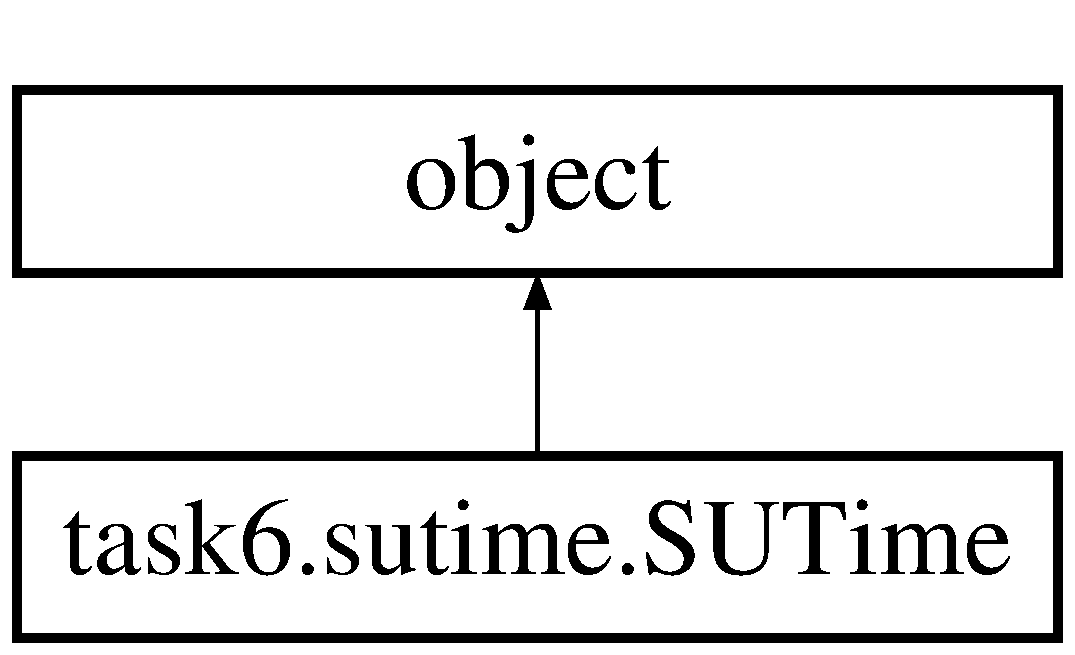
\includegraphics[height=2.000000cm]{classtask6_1_1sutime_1_1SUTime}
\end{center}
\end{figure}
\subsection*{Public Member Functions}
\begin{DoxyCompactItemize}
\item 
def \hyperlink{classtask6_1_1sutime_1_1SUTime_ad3d2f079441d91580b76c08e8cbbc01c}{\+\_\+\+\_\+init\+\_\+\+\_\+} (self, \hyperlink{classtask6_1_1sutime_1_1SUTime_aee86d05dd182246589b8f0eb6ea16897}{jars}=\mbox{[}$\,$\mbox{]}, jvm\+\_\+started=False, \hyperlink{classtask6_1_1sutime_1_1SUTime_a406b3a84a46ccab63a3b514e475d998e}{mark\+\_\+time\+\_\+ranges}=False, \hyperlink{classtask6_1_1sutime_1_1SUTime_a7e81771e26b1f92df6118f131798a034}{include\+\_\+range}=False)
\item 
def \hyperlink{classtask6_1_1sutime_1_1SUTime_a171448f34de8cab7d19e1353c8495c65}{parse} (self, input\+\_\+str, reference\+\_\+date=\textquotesingle{}\textquotesingle{})
\end{DoxyCompactItemize}
\subsection*{Public Attributes}
\begin{DoxyCompactItemize}
\item 
\hyperlink{classtask6_1_1sutime_1_1SUTime_a406b3a84a46ccab63a3b514e475d998e}{mark\+\_\+time\+\_\+ranges}
\item 
\hyperlink{classtask6_1_1sutime_1_1SUTime_a7e81771e26b1f92df6118f131798a034}{include\+\_\+range}
\item 
\hyperlink{classtask6_1_1sutime_1_1SUTime_aee86d05dd182246589b8f0eb6ea16897}{jars}
\end{DoxyCompactItemize}


\subsection{Detailed Description}
\begin{DoxyVerb}Python wrapper for SUTime (CoreNLP) by Stanford.

Attributes:
    jars: List of paths to the SUTime Java dependencies.
    jvm_started: Optional attribute to specify if the JVM has already been
        started (with all Java dependencies loaded).
    mark_time_ranges: Optional attribute to specify CoreNLP property
        sutime.markTimeRanges. Default is False.
        "Tells sutime to mark phrases such as 'From January to March'
        instead of marking 'January' and 'March' separately"
    include_range: Optional attribute to specify CoreNLP property
        sutime.includeRange. Default is False.
        "Tells sutime to mark phrases such as 'From January to March'
        instead of marking 'January' and 'March' separately"
\end{DoxyVerb}
 

Definition at line 11 of file sutime.\+py.



\subsection{Constructor \& Destructor Documentation}
\mbox{\Hypertarget{classtask6_1_1sutime_1_1SUTime_ad3d2f079441d91580b76c08e8cbbc01c}\label{classtask6_1_1sutime_1_1SUTime_ad3d2f079441d91580b76c08e8cbbc01c}} 
\index{task6\+::sutime\+::\+S\+U\+Time@{task6\+::sutime\+::\+S\+U\+Time}!\+\_\+\+\_\+init\+\_\+\+\_\+@{\+\_\+\+\_\+init\+\_\+\+\_\+}}
\index{\+\_\+\+\_\+init\+\_\+\+\_\+@{\+\_\+\+\_\+init\+\_\+\+\_\+}!task6\+::sutime\+::\+S\+U\+Time@{task6\+::sutime\+::\+S\+U\+Time}}
\subsubsection{\texorpdfstring{\+\_\+\+\_\+init\+\_\+\+\_\+()}{\_\_init\_\_()}}
{\footnotesize\ttfamily def task6.\+sutime.\+S\+U\+Time.\+\_\+\+\_\+init\+\_\+\+\_\+ (\begin{DoxyParamCaption}\item[{}]{self,  }\item[{}]{jars = {\ttfamily \mbox{[}\mbox{]}},  }\item[{}]{jvm\+\_\+started = {\ttfamily False},  }\item[{}]{mark\+\_\+time\+\_\+ranges = {\ttfamily False},  }\item[{}]{include\+\_\+range = {\ttfamily False} }\end{DoxyParamCaption})}

\begin{DoxyVerb}Initializes SUTime.
\end{DoxyVerb}
 

Definition at line 36 of file sutime.\+py.



\subsection{Member Function Documentation}
\mbox{\Hypertarget{classtask6_1_1sutime_1_1SUTime_a171448f34de8cab7d19e1353c8495c65}\label{classtask6_1_1sutime_1_1SUTime_a171448f34de8cab7d19e1353c8495c65}} 
\index{task6\+::sutime\+::\+S\+U\+Time@{task6\+::sutime\+::\+S\+U\+Time}!parse@{parse}}
\index{parse@{parse}!task6\+::sutime\+::\+S\+U\+Time@{task6\+::sutime\+::\+S\+U\+Time}}
\subsubsection{\texorpdfstring{parse()}{parse()}}
{\footnotesize\ttfamily def task6.\+sutime.\+S\+U\+Time.\+parse (\begin{DoxyParamCaption}\item[{}]{self,  }\item[{}]{input\+\_\+str,  }\item[{}]{reference\+\_\+date = {\ttfamily \textquotesingle{}\textquotesingle{}} }\end{DoxyParamCaption})}

\begin{DoxyVerb}Parses datetime information out of string input.

It invokes the SUTimeWrapper.annotate() function in Java.

Args:
    input_str: The input as string that has to be parsed.
    reference_date: Optional reference data for SUTime.

Returns:
    A list of dicts with the result from the SUTimeWrapper.annotate()
call.

Raises:
    RuntimeError: An error occurres when CoreNLP is not loaded.
\end{DoxyVerb}
 

Definition at line 95 of file sutime.\+py.



\subsection{Member Data Documentation}
\mbox{\Hypertarget{classtask6_1_1sutime_1_1SUTime_a7e81771e26b1f92df6118f131798a034}\label{classtask6_1_1sutime_1_1SUTime_a7e81771e26b1f92df6118f131798a034}} 
\index{task6\+::sutime\+::\+S\+U\+Time@{task6\+::sutime\+::\+S\+U\+Time}!include\+\_\+range@{include\+\_\+range}}
\index{include\+\_\+range@{include\+\_\+range}!task6\+::sutime\+::\+S\+U\+Time@{task6\+::sutime\+::\+S\+U\+Time}}
\subsubsection{\texorpdfstring{include\+\_\+range}{include\_range}}
{\footnotesize\ttfamily task6.\+sutime.\+S\+U\+Time.\+include\+\_\+range}



Definition at line 40 of file sutime.\+py.

\mbox{\Hypertarget{classtask6_1_1sutime_1_1SUTime_aee86d05dd182246589b8f0eb6ea16897}\label{classtask6_1_1sutime_1_1SUTime_aee86d05dd182246589b8f0eb6ea16897}} 
\index{task6\+::sutime\+::\+S\+U\+Time@{task6\+::sutime\+::\+S\+U\+Time}!jars@{jars}}
\index{jars@{jars}!task6\+::sutime\+::\+S\+U\+Time@{task6\+::sutime\+::\+S\+U\+Time}}
\subsubsection{\texorpdfstring{jars}{jars}}
{\footnotesize\ttfamily task6.\+sutime.\+S\+U\+Time.\+jars}



Definition at line 41 of file sutime.\+py.

\mbox{\Hypertarget{classtask6_1_1sutime_1_1SUTime_a406b3a84a46ccab63a3b514e475d998e}\label{classtask6_1_1sutime_1_1SUTime_a406b3a84a46ccab63a3b514e475d998e}} 
\index{task6\+::sutime\+::\+S\+U\+Time@{task6\+::sutime\+::\+S\+U\+Time}!mark\+\_\+time\+\_\+ranges@{mark\+\_\+time\+\_\+ranges}}
\index{mark\+\_\+time\+\_\+ranges@{mark\+\_\+time\+\_\+ranges}!task6\+::sutime\+::\+S\+U\+Time@{task6\+::sutime\+::\+S\+U\+Time}}
\subsubsection{\texorpdfstring{mark\+\_\+time\+\_\+ranges}{mark\_time\_ranges}}
{\footnotesize\ttfamily task6.\+sutime.\+S\+U\+Time.\+mark\+\_\+time\+\_\+ranges}



Definition at line 39 of file sutime.\+py.



The documentation for this class was generated from the following file\+:\begin{DoxyCompactItemize}
\item 
task6/\hyperlink{sutime_8py}{sutime.\+py}\end{DoxyCompactItemize}

\hypertarget{classtask6_1_1t6Entities_1_1t6Entity}{}\section{task6.\+t6\+Entities.\+t6\+Entity Class Reference}
\label{classtask6_1_1t6Entities_1_1t6Entity}\index{task6.\+t6\+Entities.\+t6\+Entity@{task6.\+t6\+Entities.\+t6\+Entity}}


Programmer Name\+: Luke Maffey Date\+: 9/19/17 Module Purpose\+: Class definitions for all Time\+Norm entities -\/ Intervals, Periods, Repeating-\/\+Intervals, and Operators.  


Inheritance diagram for task6.\+t6\+Entities.\+t6\+Entity\+:\begin{figure}[H]
\begin{center}
\leavevmode
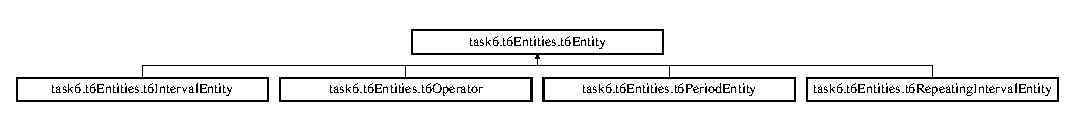
\includegraphics[height=1.138211cm]{classtask6_1_1t6Entities_1_1t6Entity}
\end{center}
\end{figure}
\subsection*{Public Member Functions}
\begin{DoxyCompactItemize}
\item 
def \hyperlink{classtask6_1_1t6Entities_1_1t6Entity_ac0bcf8dbefa28c8e1a77d891e368c9e1}{\+\_\+\+\_\+init\+\_\+\+\_\+} (self, \hyperlink{classtask6_1_1t6Entities_1_1t6Entity_a96b2e7fb553c920ab2db6f6deb31e3b4}{id}, \hyperlink{classtask6_1_1t6Entities_1_1t6Entity_a8221c36d2995a24200cdfbd74cc9233c}{start\+\_\+span}, \hyperlink{classtask6_1_1t6Entities_1_1t6Entity_a597d42bb02fc9f42277098f0ce21917c}{end\+\_\+span}, \hyperlink{classtask6_1_1t6Entities_1_1t6Entity_af0496eb852234bb168ab22d031c99ed3}{type}, \hyperlink{classtask6_1_1t6Entities_1_1t6Entity_a18ba365facb8cb062830abb11cf741f6}{parent\+\_\+type})
\item 
def \hyperlink{classtask6_1_1t6Entities_1_1t6Entity_a60cd3a7b64d13bbacb877267fa0151fe}{\+\_\+\+\_\+str\+\_\+\+\_\+} (self)
\item 
def \hyperlink{classtask6_1_1t6Entities_1_1t6Entity_a5387d85b2aa40e213b9962470207bd09}{set\+ID} (self, \hyperlink{classtask6_1_1t6Entities_1_1t6Entity_a96b2e7fb553c920ab2db6f6deb31e3b4}{id})
\item 
def \hyperlink{classtask6_1_1t6Entities_1_1t6Entity_aadb42e2b65a301043fb6162e4f14edd7}{get\+ID} (self)
\item 
def \hyperlink{classtask6_1_1t6Entities_1_1t6Entity_ae24a589eee8e89e5cc9d2116a05f574c}{print\+String} (self)
\item 
def \hyperlink{classtask6_1_1t6Entities_1_1t6Entity_ad72f67fab17e07055b34d77834174f75}{parent\+Type} (self)
\item 
def \hyperlink{classtask6_1_1t6Entities_1_1t6Entity_acd1af6b899f68fec07c9749e5d0129fa}{print\+X\+ML} (self)
\end{DoxyCompactItemize}
\subsection*{Public Attributes}
\begin{DoxyCompactItemize}
\item 
\hyperlink{classtask6_1_1t6Entities_1_1t6Entity_a96b2e7fb553c920ab2db6f6deb31e3b4}{id}
\item 
\hyperlink{classtask6_1_1t6Entities_1_1t6Entity_a8221c36d2995a24200cdfbd74cc9233c}{start\+\_\+span}
\item 
\hyperlink{classtask6_1_1t6Entities_1_1t6Entity_a597d42bb02fc9f42277098f0ce21917c}{end\+\_\+span}
\item 
\hyperlink{classtask6_1_1t6Entities_1_1t6Entity_af0496eb852234bb168ab22d031c99ed3}{type}
\item 
\hyperlink{classtask6_1_1t6Entities_1_1t6Entity_a18ba365facb8cb062830abb11cf741f6}{parent\+\_\+type}
\end{DoxyCompactItemize}


\subsection{Detailed Description}
Programmer Name\+: Luke Maffey Date\+: 9/19/17 Module Purpose\+: Class definitions for all Time\+Norm entities -\/ Intervals, Periods, Repeating-\/\+Intervals, and Operators. 

\subsection{Constructor \& Destructor Documentation}
\mbox{\Hypertarget{classtask6_1_1t6Entities_1_1t6Entity_ac0bcf8dbefa28c8e1a77d891e368c9e1}\label{classtask6_1_1t6Entities_1_1t6Entity_ac0bcf8dbefa28c8e1a77d891e368c9e1}} 
\index{task6\+::t6\+Entities\+::t6\+Entity@{task6\+::t6\+Entities\+::t6\+Entity}!\+\_\+\+\_\+init\+\_\+\+\_\+@{\+\_\+\+\_\+init\+\_\+\+\_\+}}
\index{\+\_\+\+\_\+init\+\_\+\+\_\+@{\+\_\+\+\_\+init\+\_\+\+\_\+}!task6\+::t6\+Entities\+::t6\+Entity@{task6\+::t6\+Entities\+::t6\+Entity}}
\subsubsection{\texorpdfstring{\+\_\+\+\_\+init\+\_\+\+\_\+()}{\_\_init\_\_()}}
{\footnotesize\ttfamily def task6.\+t6\+Entities.\+t6\+Entity.\+\_\+\+\_\+init\+\_\+\+\_\+ (\begin{DoxyParamCaption}\item[{}]{self,  }\item[{}]{id,  }\item[{}]{start\+\_\+span,  }\item[{}]{end\+\_\+span,  }\item[{}]{type,  }\item[{}]{parent\+\_\+type }\end{DoxyParamCaption})}



\subsection{Member Function Documentation}
\mbox{\Hypertarget{classtask6_1_1t6Entities_1_1t6Entity_a60cd3a7b64d13bbacb877267fa0151fe}\label{classtask6_1_1t6Entities_1_1t6Entity_a60cd3a7b64d13bbacb877267fa0151fe}} 
\index{task6\+::t6\+Entities\+::t6\+Entity@{task6\+::t6\+Entities\+::t6\+Entity}!\+\_\+\+\_\+str\+\_\+\+\_\+@{\+\_\+\+\_\+str\+\_\+\+\_\+}}
\index{\+\_\+\+\_\+str\+\_\+\+\_\+@{\+\_\+\+\_\+str\+\_\+\+\_\+}!task6\+::t6\+Entities\+::t6\+Entity@{task6\+::t6\+Entities\+::t6\+Entity}}
\subsubsection{\texorpdfstring{\+\_\+\+\_\+str\+\_\+\+\_\+()}{\_\_str\_\_()}}
{\footnotesize\ttfamily def task6.\+t6\+Entities.\+t6\+Entity.\+\_\+\+\_\+str\+\_\+\+\_\+ (\begin{DoxyParamCaption}\item[{}]{self }\end{DoxyParamCaption})}

\mbox{\Hypertarget{classtask6_1_1t6Entities_1_1t6Entity_aadb42e2b65a301043fb6162e4f14edd7}\label{classtask6_1_1t6Entities_1_1t6Entity_aadb42e2b65a301043fb6162e4f14edd7}} 
\index{task6\+::t6\+Entities\+::t6\+Entity@{task6\+::t6\+Entities\+::t6\+Entity}!get\+ID@{get\+ID}}
\index{get\+ID@{get\+ID}!task6\+::t6\+Entities\+::t6\+Entity@{task6\+::t6\+Entities\+::t6\+Entity}}
\subsubsection{\texorpdfstring{get\+I\+D()}{getID()}}
{\footnotesize\ttfamily def task6.\+t6\+Entities.\+t6\+Entity.\+get\+ID (\begin{DoxyParamCaption}\item[{}]{self }\end{DoxyParamCaption})}

\mbox{\Hypertarget{classtask6_1_1t6Entities_1_1t6Entity_ad72f67fab17e07055b34d77834174f75}\label{classtask6_1_1t6Entities_1_1t6Entity_ad72f67fab17e07055b34d77834174f75}} 
\index{task6\+::t6\+Entities\+::t6\+Entity@{task6\+::t6\+Entities\+::t6\+Entity}!parent\+Type@{parent\+Type}}
\index{parent\+Type@{parent\+Type}!task6\+::t6\+Entities\+::t6\+Entity@{task6\+::t6\+Entities\+::t6\+Entity}}
\subsubsection{\texorpdfstring{parent\+Type()}{parentType()}}
{\footnotesize\ttfamily def task6.\+t6\+Entities.\+t6\+Entity.\+parent\+Type (\begin{DoxyParamCaption}\item[{}]{self }\end{DoxyParamCaption})}

\mbox{\Hypertarget{classtask6_1_1t6Entities_1_1t6Entity_ae24a589eee8e89e5cc9d2116a05f574c}\label{classtask6_1_1t6Entities_1_1t6Entity_ae24a589eee8e89e5cc9d2116a05f574c}} 
\index{task6\+::t6\+Entities\+::t6\+Entity@{task6\+::t6\+Entities\+::t6\+Entity}!print\+String@{print\+String}}
\index{print\+String@{print\+String}!task6\+::t6\+Entities\+::t6\+Entity@{task6\+::t6\+Entities\+::t6\+Entity}}
\subsubsection{\texorpdfstring{print\+String()}{printString()}}
{\footnotesize\ttfamily def task6.\+t6\+Entities.\+t6\+Entity.\+print\+String (\begin{DoxyParamCaption}\item[{}]{self }\end{DoxyParamCaption})}

\mbox{\Hypertarget{classtask6_1_1t6Entities_1_1t6Entity_acd1af6b899f68fec07c9749e5d0129fa}\label{classtask6_1_1t6Entities_1_1t6Entity_acd1af6b899f68fec07c9749e5d0129fa}} 
\index{task6\+::t6\+Entities\+::t6\+Entity@{task6\+::t6\+Entities\+::t6\+Entity}!print\+X\+ML@{print\+X\+ML}}
\index{print\+X\+ML@{print\+X\+ML}!task6\+::t6\+Entities\+::t6\+Entity@{task6\+::t6\+Entities\+::t6\+Entity}}
\subsubsection{\texorpdfstring{print\+X\+M\+L()}{printXML()}}
{\footnotesize\ttfamily def task6.\+t6\+Entities.\+t6\+Entity.\+print\+X\+ML (\begin{DoxyParamCaption}\item[{}]{self }\end{DoxyParamCaption})}

\mbox{\Hypertarget{classtask6_1_1t6Entities_1_1t6Entity_a5387d85b2aa40e213b9962470207bd09}\label{classtask6_1_1t6Entities_1_1t6Entity_a5387d85b2aa40e213b9962470207bd09}} 
\index{task6\+::t6\+Entities\+::t6\+Entity@{task6\+::t6\+Entities\+::t6\+Entity}!set\+ID@{set\+ID}}
\index{set\+ID@{set\+ID}!task6\+::t6\+Entities\+::t6\+Entity@{task6\+::t6\+Entities\+::t6\+Entity}}
\subsubsection{\texorpdfstring{set\+I\+D()}{setID()}}
{\footnotesize\ttfamily def task6.\+t6\+Entities.\+t6\+Entity.\+set\+ID (\begin{DoxyParamCaption}\item[{}]{self,  }\item[{}]{id }\end{DoxyParamCaption})}



\subsection{Member Data Documentation}
\mbox{\Hypertarget{classtask6_1_1t6Entities_1_1t6Entity_a597d42bb02fc9f42277098f0ce21917c}\label{classtask6_1_1t6Entities_1_1t6Entity_a597d42bb02fc9f42277098f0ce21917c}} 
\index{task6\+::t6\+Entities\+::t6\+Entity@{task6\+::t6\+Entities\+::t6\+Entity}!end\+\_\+span@{end\+\_\+span}}
\index{end\+\_\+span@{end\+\_\+span}!task6\+::t6\+Entities\+::t6\+Entity@{task6\+::t6\+Entities\+::t6\+Entity}}
\subsubsection{\texorpdfstring{end\+\_\+span}{end\_span}}
{\footnotesize\ttfamily task6.\+t6\+Entities.\+t6\+Entity.\+end\+\_\+span}

\mbox{\Hypertarget{classtask6_1_1t6Entities_1_1t6Entity_a96b2e7fb553c920ab2db6f6deb31e3b4}\label{classtask6_1_1t6Entities_1_1t6Entity_a96b2e7fb553c920ab2db6f6deb31e3b4}} 
\index{task6\+::t6\+Entities\+::t6\+Entity@{task6\+::t6\+Entities\+::t6\+Entity}!id@{id}}
\index{id@{id}!task6\+::t6\+Entities\+::t6\+Entity@{task6\+::t6\+Entities\+::t6\+Entity}}
\subsubsection{\texorpdfstring{id}{id}}
{\footnotesize\ttfamily task6.\+t6\+Entities.\+t6\+Entity.\+id}

\mbox{\Hypertarget{classtask6_1_1t6Entities_1_1t6Entity_a18ba365facb8cb062830abb11cf741f6}\label{classtask6_1_1t6Entities_1_1t6Entity_a18ba365facb8cb062830abb11cf741f6}} 
\index{task6\+::t6\+Entities\+::t6\+Entity@{task6\+::t6\+Entities\+::t6\+Entity}!parent\+\_\+type@{parent\+\_\+type}}
\index{parent\+\_\+type@{parent\+\_\+type}!task6\+::t6\+Entities\+::t6\+Entity@{task6\+::t6\+Entities\+::t6\+Entity}}
\subsubsection{\texorpdfstring{parent\+\_\+type}{parent\_type}}
{\footnotesize\ttfamily task6.\+t6\+Entities.\+t6\+Entity.\+parent\+\_\+type}

\mbox{\Hypertarget{classtask6_1_1t6Entities_1_1t6Entity_a8221c36d2995a24200cdfbd74cc9233c}\label{classtask6_1_1t6Entities_1_1t6Entity_a8221c36d2995a24200cdfbd74cc9233c}} 
\index{task6\+::t6\+Entities\+::t6\+Entity@{task6\+::t6\+Entities\+::t6\+Entity}!start\+\_\+span@{start\+\_\+span}}
\index{start\+\_\+span@{start\+\_\+span}!task6\+::t6\+Entities\+::t6\+Entity@{task6\+::t6\+Entities\+::t6\+Entity}}
\subsubsection{\texorpdfstring{start\+\_\+span}{start\_span}}
{\footnotesize\ttfamily task6.\+t6\+Entities.\+t6\+Entity.\+start\+\_\+span}

\mbox{\Hypertarget{classtask6_1_1t6Entities_1_1t6Entity_af0496eb852234bb168ab22d031c99ed3}\label{classtask6_1_1t6Entities_1_1t6Entity_af0496eb852234bb168ab22d031c99ed3}} 
\index{task6\+::t6\+Entities\+::t6\+Entity@{task6\+::t6\+Entities\+::t6\+Entity}!type@{type}}
\index{type@{type}!task6\+::t6\+Entities\+::t6\+Entity@{task6\+::t6\+Entities\+::t6\+Entity}}
\subsubsection{\texorpdfstring{type}{type}}
{\footnotesize\ttfamily task6.\+t6\+Entities.\+t6\+Entity.\+type}



The documentation for this class was generated from the following file\+:\begin{DoxyCompactItemize}
\item 
task6/\hyperlink{t6Entities_8py}{t6\+Entities.\+py}\end{DoxyCompactItemize}

\hypertarget{classtask6_1_1t6Entities_1_1t6IntervalEntity}{}\section{task6.\+t6\+Entities.\+t6\+Interval\+Entity Class Reference}
\label{classtask6_1_1t6Entities_1_1t6IntervalEntity}\index{task6.\+t6\+Entities.\+t6\+Interval\+Entity@{task6.\+t6\+Entities.\+t6\+Interval\+Entity}}
Inheritance diagram for task6.\+t6\+Entities.\+t6\+Interval\+Entity\+:\begin{figure}[H]
\begin{center}
\leavevmode
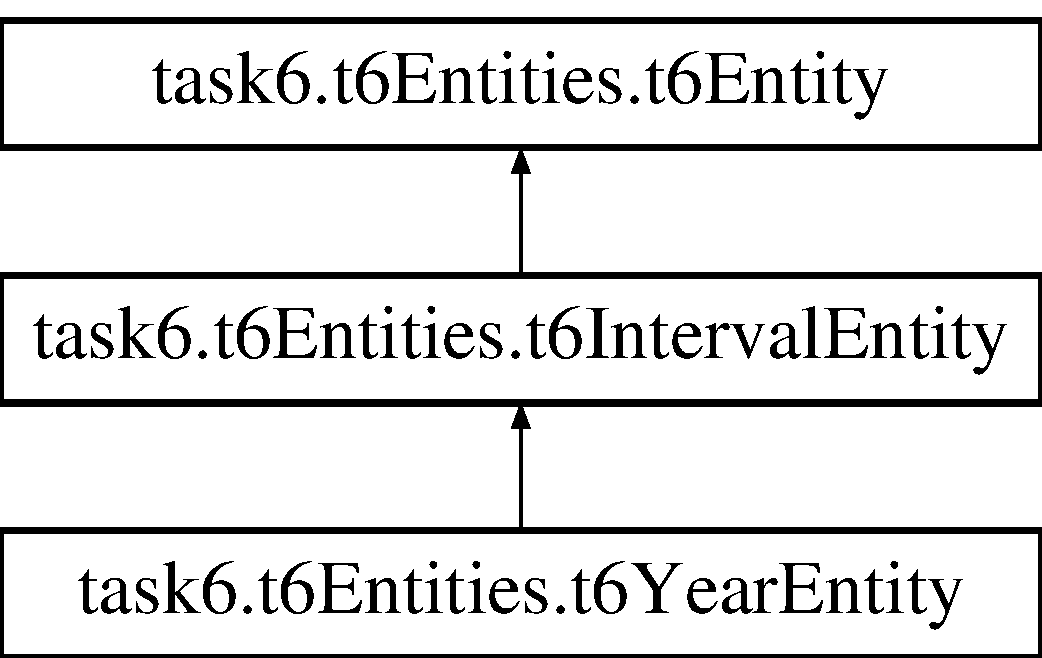
\includegraphics[height=2.000000cm]{classtask6_1_1t6Entities_1_1t6IntervalEntity}
\end{center}
\end{figure}
\subsection*{Public Member Functions}
\begin{DoxyCompactItemize}
\item 
def \hyperlink{classtask6_1_1t6Entities_1_1t6IntervalEntity_a1ac32d786c2759c6886bcde28846eb0d}{\+\_\+\+\_\+init\+\_\+\+\_\+} (self, \hyperlink{classtask6_1_1t6Entities_1_1t6Entity_a96b2e7fb553c920ab2db6f6deb31e3b4}{id}, \hyperlink{classtask6_1_1t6Entities_1_1t6Entity_a8221c36d2995a24200cdfbd74cc9233c}{start\+\_\+span}, \hyperlink{classtask6_1_1t6Entities_1_1t6Entity_a597d42bb02fc9f42277098f0ce21917c}{end\+\_\+span}, \hyperlink{classtask6_1_1t6Entities_1_1t6IntervalEntity_a002714e201e05948aca8cce83d4a9da6}{value})
\end{DoxyCompactItemize}
\subsection*{Public Attributes}
\begin{DoxyCompactItemize}
\item 
\hyperlink{classtask6_1_1t6Entities_1_1t6IntervalEntity_a002714e201e05948aca8cce83d4a9da6}{value}
\end{DoxyCompactItemize}


\subsection{Detailed Description}


Definition at line 33 of file t6\+Entities.\+py.



\subsection{Constructor \& Destructor Documentation}
\mbox{\Hypertarget{classtask6_1_1t6Entities_1_1t6IntervalEntity_a1ac32d786c2759c6886bcde28846eb0d}\label{classtask6_1_1t6Entities_1_1t6IntervalEntity_a1ac32d786c2759c6886bcde28846eb0d}} 
\index{task6\+::t6\+Entities\+::t6\+Interval\+Entity@{task6\+::t6\+Entities\+::t6\+Interval\+Entity}!\+\_\+\+\_\+init\+\_\+\+\_\+@{\+\_\+\+\_\+init\+\_\+\+\_\+}}
\index{\+\_\+\+\_\+init\+\_\+\+\_\+@{\+\_\+\+\_\+init\+\_\+\+\_\+}!task6\+::t6\+Entities\+::t6\+Interval\+Entity@{task6\+::t6\+Entities\+::t6\+Interval\+Entity}}
\subsubsection{\texorpdfstring{\+\_\+\+\_\+init\+\_\+\+\_\+()}{\_\_init\_\_()}}
{\footnotesize\ttfamily def task6.\+t6\+Entities.\+t6\+Interval\+Entity.\+\_\+\+\_\+init\+\_\+\+\_\+ (\begin{DoxyParamCaption}\item[{}]{self,  }\item[{}]{id,  }\item[{}]{start\+\_\+span,  }\item[{}]{end\+\_\+span,  }\item[{}]{value }\end{DoxyParamCaption})}



Definition at line 34 of file t6\+Entities.\+py.



\subsection{Member Data Documentation}
\mbox{\Hypertarget{classtask6_1_1t6Entities_1_1t6IntervalEntity_a002714e201e05948aca8cce83d4a9da6}\label{classtask6_1_1t6Entities_1_1t6IntervalEntity_a002714e201e05948aca8cce83d4a9da6}} 
\index{task6\+::t6\+Entities\+::t6\+Interval\+Entity@{task6\+::t6\+Entities\+::t6\+Interval\+Entity}!value@{value}}
\index{value@{value}!task6\+::t6\+Entities\+::t6\+Interval\+Entity@{task6\+::t6\+Entities\+::t6\+Interval\+Entity}}
\subsubsection{\texorpdfstring{value}{value}}
{\footnotesize\ttfamily task6.\+t6\+Entities.\+t6\+Interval\+Entity.\+value}



Definition at line 36 of file t6\+Entities.\+py.



The documentation for this class was generated from the following file\+:\begin{DoxyCompactItemize}
\item 
task6/\hyperlink{t6Entities_8py}{t6\+Entities.\+py}\end{DoxyCompactItemize}

\hypertarget{classtask6_1_1t6Entities_1_1t6Operator}{}\section{task6.\+t6\+Entities.\+t6\+Operator Class Reference}
\label{classtask6_1_1t6Entities_1_1t6Operator}\index{task6.\+t6\+Entities.\+t6\+Operator@{task6.\+t6\+Entities.\+t6\+Operator}}
Inheritance diagram for task6.\+t6\+Entities.\+t6\+Operator\+:\begin{figure}[H]
\begin{center}
\leavevmode
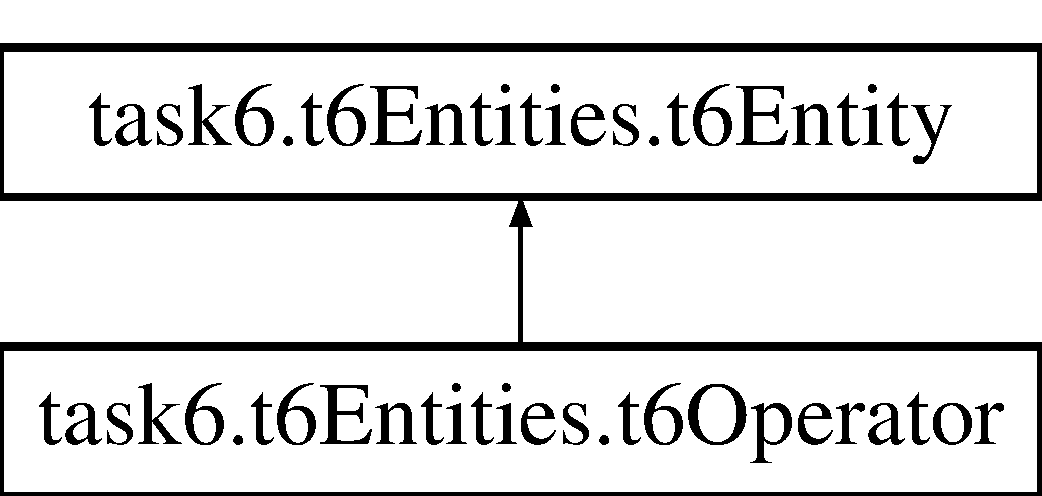
\includegraphics[height=2.000000cm]{classtask6_1_1t6Entities_1_1t6Operator}
\end{center}
\end{figure}
\subsection*{Public Member Functions}
\begin{DoxyCompactItemize}
\item 
def \hyperlink{classtask6_1_1t6Entities_1_1t6Operator_a742bafc1cb775d74ee2be13f8c880472}{\+\_\+\+\_\+init\+\_\+\+\_\+} (self, \hyperlink{classtask6_1_1t6Entities_1_1t6Entity_a96b2e7fb553c920ab2db6f6deb31e3b4}{id}, \hyperlink{classtask6_1_1t6Entities_1_1t6Entity_a8221c36d2995a24200cdfbd74cc9233c}{start\+\_\+span}, \hyperlink{classtask6_1_1t6Entities_1_1t6Entity_a597d42bb02fc9f42277098f0ce21917c}{end\+\_\+span}, operator\+Type)
\end{DoxyCompactItemize}
\subsection*{Additional Inherited Members}


\subsection{Detailed Description}


Definition at line 158 of file t6\+Entities.\+py.



\subsection{Constructor \& Destructor Documentation}
\mbox{\Hypertarget{classtask6_1_1t6Entities_1_1t6Operator_a742bafc1cb775d74ee2be13f8c880472}\label{classtask6_1_1t6Entities_1_1t6Operator_a742bafc1cb775d74ee2be13f8c880472}} 
\index{task6\+::t6\+Entities\+::t6\+Operator@{task6\+::t6\+Entities\+::t6\+Operator}!\+\_\+\+\_\+init\+\_\+\+\_\+@{\+\_\+\+\_\+init\+\_\+\+\_\+}}
\index{\+\_\+\+\_\+init\+\_\+\+\_\+@{\+\_\+\+\_\+init\+\_\+\+\_\+}!task6\+::t6\+Entities\+::t6\+Operator@{task6\+::t6\+Entities\+::t6\+Operator}}
\subsubsection{\texorpdfstring{\+\_\+\+\_\+init\+\_\+\+\_\+()}{\_\_init\_\_()}}
{\footnotesize\ttfamily def task6.\+t6\+Entities.\+t6\+Operator.\+\_\+\+\_\+init\+\_\+\+\_\+ (\begin{DoxyParamCaption}\item[{}]{self,  }\item[{}]{id,  }\item[{}]{start\+\_\+span,  }\item[{}]{end\+\_\+span,  }\item[{}]{operator\+Type }\end{DoxyParamCaption})}



Definition at line 159 of file t6\+Entities.\+py.



The documentation for this class was generated from the following file\+:\begin{DoxyCompactItemize}
\item 
task6/\hyperlink{t6Entities_8py}{t6\+Entities.\+py}\end{DoxyCompactItemize}

\hypertarget{classtask6_1_1t6Entities_1_1t6PeriodEntity}{}\section{task6.\+t6\+Entities.\+t6\+Period\+Entity Class Reference}
\label{classtask6_1_1t6Entities_1_1t6PeriodEntity}\index{task6.\+t6\+Entities.\+t6\+Period\+Entity@{task6.\+t6\+Entities.\+t6\+Period\+Entity}}
Inheritance diagram for task6.\+t6\+Entities.\+t6\+Period\+Entity\+:\begin{figure}[H]
\begin{center}
\leavevmode
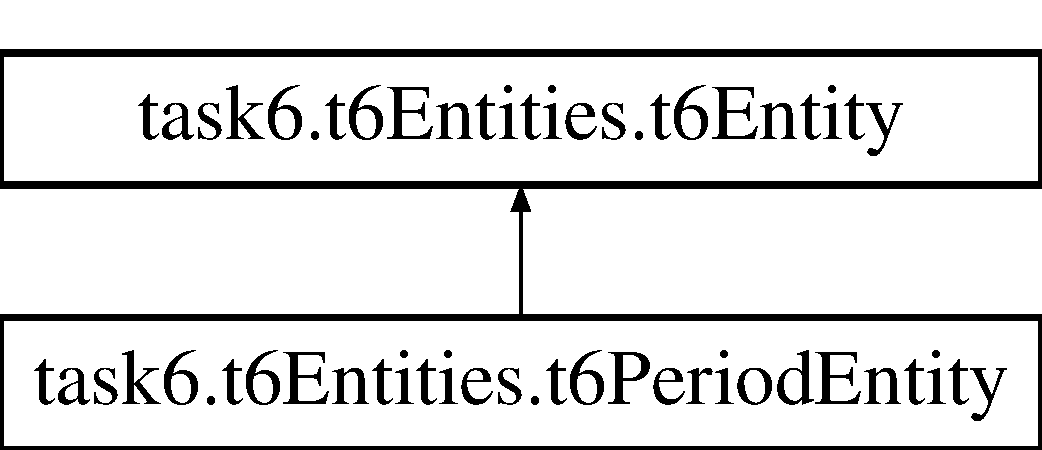
\includegraphics[height=2.000000cm]{classtask6_1_1t6Entities_1_1t6PeriodEntity}
\end{center}
\end{figure}
\subsection*{Public Member Functions}
\begin{DoxyCompactItemize}
\item 
def \hyperlink{classtask6_1_1t6Entities_1_1t6PeriodEntity_a447a8538b93c2116de30aa47eccfcbec}{\+\_\+\+\_\+init\+\_\+\+\_\+} (self, \hyperlink{classtask6_1_1t6Entities_1_1t6Entity_a96b2e7fb553c920ab2db6f6deb31e3b4}{id}, \hyperlink{classtask6_1_1t6Entities_1_1t6Entity_a8221c36d2995a24200cdfbd74cc9233c}{start\+\_\+span}, \hyperlink{classtask6_1_1t6Entities_1_1t6Entity_a597d42bb02fc9f42277098f0ce21917c}{end\+\_\+span}, \hyperlink{classtask6_1_1t6Entities_1_1t6PeriodEntity_ae2f4d463fe5601083ce5ce3070690f1d}{period\+Type})
\end{DoxyCompactItemize}
\subsection*{Public Attributes}
\begin{DoxyCompactItemize}
\item 
\hyperlink{classtask6_1_1t6Entities_1_1t6PeriodEntity_ae2f4d463fe5601083ce5ce3070690f1d}{period\+Type}
\end{DoxyCompactItemize}


\subsection{Detailed Description}


Definition at line 38 of file t6\+Entities.\+py.



\subsection{Constructor \& Destructor Documentation}
\mbox{\Hypertarget{classtask6_1_1t6Entities_1_1t6PeriodEntity_a447a8538b93c2116de30aa47eccfcbec}\label{classtask6_1_1t6Entities_1_1t6PeriodEntity_a447a8538b93c2116de30aa47eccfcbec}} 
\index{task6\+::t6\+Entities\+::t6\+Period\+Entity@{task6\+::t6\+Entities\+::t6\+Period\+Entity}!\+\_\+\+\_\+init\+\_\+\+\_\+@{\+\_\+\+\_\+init\+\_\+\+\_\+}}
\index{\+\_\+\+\_\+init\+\_\+\+\_\+@{\+\_\+\+\_\+init\+\_\+\+\_\+}!task6\+::t6\+Entities\+::t6\+Period\+Entity@{task6\+::t6\+Entities\+::t6\+Period\+Entity}}
\subsubsection{\texorpdfstring{\+\_\+\+\_\+init\+\_\+\+\_\+()}{\_\_init\_\_()}}
{\footnotesize\ttfamily def task6.\+t6\+Entities.\+t6\+Period\+Entity.\+\_\+\+\_\+init\+\_\+\+\_\+ (\begin{DoxyParamCaption}\item[{}]{self,  }\item[{}]{id,  }\item[{}]{start\+\_\+span,  }\item[{}]{end\+\_\+span,  }\item[{}]{period\+Type }\end{DoxyParamCaption})}



Definition at line 39 of file t6\+Entities.\+py.



\subsection{Member Data Documentation}
\mbox{\Hypertarget{classtask6_1_1t6Entities_1_1t6PeriodEntity_ae2f4d463fe5601083ce5ce3070690f1d}\label{classtask6_1_1t6Entities_1_1t6PeriodEntity_ae2f4d463fe5601083ce5ce3070690f1d}} 
\index{task6\+::t6\+Entities\+::t6\+Period\+Entity@{task6\+::t6\+Entities\+::t6\+Period\+Entity}!period\+Type@{period\+Type}}
\index{period\+Type@{period\+Type}!task6\+::t6\+Entities\+::t6\+Period\+Entity@{task6\+::t6\+Entities\+::t6\+Period\+Entity}}
\subsubsection{\texorpdfstring{period\+Type}{periodType}}
{\footnotesize\ttfamily task6.\+t6\+Entities.\+t6\+Period\+Entity.\+period\+Type}



Definition at line 41 of file t6\+Entities.\+py.



The documentation for this class was generated from the following file\+:\begin{DoxyCompactItemize}
\item 
task6/\hyperlink{t6Entities_8py}{t6\+Entities.\+py}\end{DoxyCompactItemize}

\hypertarget{classtask6_1_1t6Entities_1_1t6RepeatingIntervalEntity}{}\section{task6.\+t6\+Entities.\+t6\+Repeating\+Interval\+Entity Class Reference}
\label{classtask6_1_1t6Entities_1_1t6RepeatingIntervalEntity}\index{task6.\+t6\+Entities.\+t6\+Repeating\+Interval\+Entity@{task6.\+t6\+Entities.\+t6\+Repeating\+Interval\+Entity}}
Inheritance diagram for task6.\+t6\+Entities.\+t6\+Repeating\+Interval\+Entity\+:\begin{figure}[H]
\begin{center}
\leavevmode
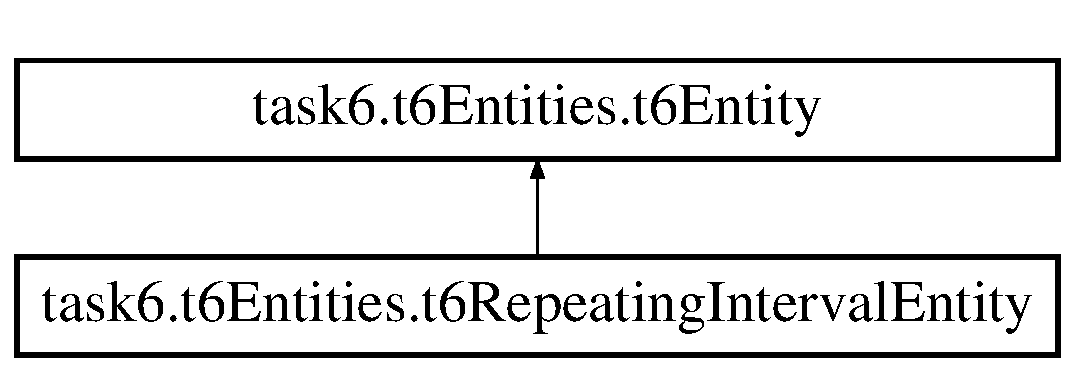
\includegraphics[height=12.000000cm]{classtask6_1_1t6Entities_1_1t6RepeatingIntervalEntity}
\end{center}
\end{figure}
\subsection*{Public Member Functions}
\begin{DoxyCompactItemize}
\item 
def \hyperlink{classtask6_1_1t6Entities_1_1t6RepeatingIntervalEntity_a2b821296d1afa9e5d79e3082a11e27d6}{\+\_\+\+\_\+init\+\_\+\+\_\+} (self, \hyperlink{classtask6_1_1t6Entities_1_1t6Entity_a96b2e7fb553c920ab2db6f6deb31e3b4}{id}, \hyperlink{classtask6_1_1t6Entities_1_1t6Entity_a8221c36d2995a24200cdfbd74cc9233c}{start\+\_\+span}, \hyperlink{classtask6_1_1t6Entities_1_1t6Entity_a597d42bb02fc9f42277098f0ce21917c}{end\+\_\+span}, \hyperlink{classtask6_1_1t6Entities_1_1t6Entity_af0496eb852234bb168ab22d031c99ed3}{type})
\end{DoxyCompactItemize}
\subsection*{Additional Inherited Members}


\subsection{Detailed Description}


Definition at line 73 of file t6\+Entities.\+py.



\subsection{Constructor \& Destructor Documentation}
\mbox{\Hypertarget{classtask6_1_1t6Entities_1_1t6RepeatingIntervalEntity_a2b821296d1afa9e5d79e3082a11e27d6}\label{classtask6_1_1t6Entities_1_1t6RepeatingIntervalEntity_a2b821296d1afa9e5d79e3082a11e27d6}} 
\index{task6\+::t6\+Entities\+::t6\+Repeating\+Interval\+Entity@{task6\+::t6\+Entities\+::t6\+Repeating\+Interval\+Entity}!\+\_\+\+\_\+init\+\_\+\+\_\+@{\+\_\+\+\_\+init\+\_\+\+\_\+}}
\index{\+\_\+\+\_\+init\+\_\+\+\_\+@{\+\_\+\+\_\+init\+\_\+\+\_\+}!task6\+::t6\+Entities\+::t6\+Repeating\+Interval\+Entity@{task6\+::t6\+Entities\+::t6\+Repeating\+Interval\+Entity}}
\subsubsection{\texorpdfstring{\+\_\+\+\_\+init\+\_\+\+\_\+()}{\_\_init\_\_()}}
{\footnotesize\ttfamily def task6.\+t6\+Entities.\+t6\+Repeating\+Interval\+Entity.\+\_\+\+\_\+init\+\_\+\+\_\+ (\begin{DoxyParamCaption}\item[{}]{self,  }\item[{}]{id,  }\item[{}]{start\+\_\+span,  }\item[{}]{end\+\_\+span,  }\item[{}]{type }\end{DoxyParamCaption})}



Definition at line 74 of file t6\+Entities.\+py.



The documentation for this class was generated from the following file\+:\begin{DoxyCompactItemize}
\item 
task6/\hyperlink{t6Entities_8py}{t6\+Entities.\+py}\end{DoxyCompactItemize}

\chapter{File Documentation}
\hypertarget{README_8md}{}\section{R\+E\+A\+D\+M\+E.\+md File Reference}
\label{README_8md}\index{R\+E\+A\+D\+M\+E.\+md@{R\+E\+A\+D\+M\+E.\+md}}

\hypertarget{setup_8py}{}\section{setup.\+py File Reference}
\label{setup_8py}\index{setup.\+py@{setup.\+py}}
\subsection*{Namespaces}
\begin{DoxyCompactItemize}
\item 
 \hyperlink{namespacesetup}{setup}
\end{DoxyCompactItemize}
\subsection*{Variables}
\begin{DoxyCompactItemize}
\item 
\hyperlink{namespacesetup_a9c076537d899ffd8096e58c282bb7b02}{setup.\+here} = path.\+abspath(path.\+dirname(\+\_\+\+\_\+file\+\_\+\+\_\+))
\item 
\hyperlink{namespacesetup_a443be2d01fd539bf6761aff70724d876}{setup.\+encoding}
\item 
\hyperlink{namespacesetup_a4cda9dbfb952875376a0749fe08a5bde}{setup.\+long\+\_\+description} = f.\+read()
\item 
\hyperlink{namespacesetup_ab3a7a0638d76a01367c5bc3cc699447f}{setup.\+name}
\item 
\hyperlink{namespacesetup_a2aa722b36a933088812b50ea79b97a5c}{setup.\+version}
\item 
\hyperlink{namespacesetup_aedf461ec52a946bda975938ba0b93ec0}{setup.\+description}
\item 
\hyperlink{namespacesetup_afc13124aa5c0124e84e1d965e3f4b0fb}{setup.\+url}
\item 
\hyperlink{namespacesetup_a3a57a4772d418a06835249cbade0d86a}{setup.\+author}
\item 
\hyperlink{namespacesetup_a5b08034343aa2be607722a8b315f3625}{setup.\+author\+\_\+email}
\item 
\hyperlink{namespacesetup_a8ed6f50a28bd6a8794f8e1153baa6de9}{setup.\+license}
\item 
\hyperlink{namespacesetup_abe96a9c38c1c61f9f0fdb002c482f785}{setup.\+classifiers}
\item 
\hyperlink{namespacesetup_a73ae9ecb109f0dcab6f0b6a89043c5c3}{setup.\+keywords}
\item 
\hyperlink{namespacesetup_aff2375a361fd5865c77bd9aa093be747}{setup.\+packages}
\item 
\hyperlink{namespacesetup_abead4f26b530856f858f0d44c7cf2588}{setup.\+install\+\_\+requires}
\end{DoxyCompactItemize}

\hypertarget{task6_2____init_____8py}{}\section{task6/\+\_\+\+\_\+init\+\_\+\+\_\+.py File Reference}
\label{task6_2____init_____8py}\index{task6/\+\_\+\+\_\+init\+\_\+\+\_\+.\+py@{task6/\+\_\+\+\_\+init\+\_\+\+\_\+.\+py}}
\subsection*{Namespaces}
\begin{DoxyCompactItemize}
\item 
 \hyperlink{namespacetask6}{task6}
\end{DoxyCompactItemize}

\hypertarget{test_2____init_____8py}{}\section{test/\+\_\+\+\_\+init\+\_\+\+\_\+.py File Reference}
\label{test_2____init_____8py}\index{test/\+\_\+\+\_\+init\+\_\+\+\_\+.\+py@{test/\+\_\+\+\_\+init\+\_\+\+\_\+.\+py}}
\subsection*{Namespaces}
\begin{DoxyCompactItemize}
\item 
 \hyperlink{namespacetest}{test}
\end{DoxyCompactItemize}

\hypertarget{sutime_8py}{}\section{task6/sutime.py File Reference}
\label{sutime_8py}\index{task6/sutime.\+py@{task6/sutime.\+py}}
\subsection*{Classes}
\begin{DoxyCompactItemize}
\item 
class \hyperlink{classtask6_1_1sutime_1_1SUTime}{task6.\+sutime.\+S\+U\+Time}
\end{DoxyCompactItemize}
\subsection*{Namespaces}
\begin{DoxyCompactItemize}
\item 
 \hyperlink{namespacetask6_1_1sutime}{task6.\+sutime}
\end{DoxyCompactItemize}

\hypertarget{sutime__wrapper_8py}{}\section{task6/sutime\+\_\+wrapper.py File Reference}
\label{sutime__wrapper_8py}\index{task6/sutime\+\_\+wrapper.\+py@{task6/sutime\+\_\+wrapper.\+py}}
\subsection*{Namespaces}
\begin{DoxyCompactItemize}
\item 
 \hyperlink{namespacetask6_1_1sutime__wrapper}{task6.\+sutime\+\_\+wrapper}
\end{DoxyCompactItemize}
\subsection*{Functions}
\begin{DoxyCompactItemize}
\item 
def \hyperlink{namespacetask6_1_1sutime__wrapper_af4cac751d594757efbe539a28850ff28}{task6.\+sutime\+\_\+wrapper.\+call\+S\+U\+Time\+Parse} (file\+\_\+path)
\begin{DoxyCompactList}\small\item\em call\+S\+U\+T\+I\+M\+E\+Parse() Function Purpose\+: Takes in raw text file and performs S\+U\+Time\textquotesingle{}s algorithm on \#it and returns it in J\+S\+ON format. \end{DoxyCompactList}\end{DoxyCompactItemize}

\hypertarget{t6Entities_8py}{}\section{task6/t6\+Entities.py File Reference}
\label{t6Entities_8py}\index{task6/t6\+Entities.\+py@{task6/t6\+Entities.\+py}}
\subsection*{Classes}
\begin{DoxyCompactItemize}
\item 
class \hyperlink{classtask6_1_1t6Entities_1_1t6Entity}{task6.\+t6\+Entities.\+t6\+Entity}
\begin{DoxyCompactList}\small\item\em Programmer Name\+: Luke Maffey Date\+: 9/19/17 Module Purpose\+: Class definitions for all Time\+Norm entities -\/ Intervals, Periods, Repeating-\/\+Intervals, and Operators. \end{DoxyCompactList}\item 
class \hyperlink{classtask6_1_1t6Entities_1_1t6IntervalEntity}{task6.\+t6\+Entities.\+t6\+Interval\+Entity}
\item 
class \hyperlink{classtask6_1_1t6Entities_1_1t6PeriodEntity}{task6.\+t6\+Entities.\+t6\+Period\+Entity}
\item 
class \hyperlink{classtask6_1_1t6Entities_1_1t6RepeatingIntervalEntity}{task6.\+t6\+Entities.\+t6\+Repeating\+Interval\+Entity}
\item 
class \hyperlink{classtask6_1_1t6Entities_1_1t6Operator}{task6.\+t6\+Entities.\+t6\+Operator}
\end{DoxyCompactItemize}
\subsection*{Namespaces}
\begin{DoxyCompactItemize}
\item 
 \hyperlink{namespacetask6_1_1t6Entities}{task6.\+t6\+Entities}
\end{DoxyCompactItemize}

\hypertarget{utils_8py}{}\section{task6/utils.py File Reference}
\label{utils_8py}\index{task6/utils.\+py@{task6/utils.\+py}}
\subsection*{Namespaces}
\begin{DoxyCompactItemize}
\item 
 \hyperlink{namespacetask6_1_1utils}{task6.\+utils}
\end{DoxyCompactItemize}
\subsection*{Functions}
\begin{DoxyCompactItemize}
\item 
def \hyperlink{namespacetask6_1_1utils_a515e86e4cb66853a491562c4dd7935b1}{task6.\+utils.\+get\+Whitespace\+Spans} (file\+\_\+path)
\begin{DoxyCompactList}\small\item\em \hyperlink{namespacetask6_1_1utils_a515e86e4cb66853a491562c4dd7935b1}{get\+Whitespace\+Spans()} Function Purpose\+: Pasrses a text file to idenitfy all tokens seperated by white space with their original file span coordinates. \end{DoxyCompactList}\end{DoxyCompactItemize}

\hypertarget{test_2test_8py}{}\section{test/test.py File Reference}
\label{test_2test_8py}\index{test/test.\+py@{test/test.\+py}}
\subsection*{Namespaces}
\begin{DoxyCompactItemize}
\item 
 \hyperlink{namespacetest_1_1test}{test.\+test}
\end{DoxyCompactItemize}
\subsection*{Variables}
\begin{DoxyCompactItemize}
\item 
\hyperlink{namespacetest_1_1test_ac6940ca06224277c08c299101b3296b4}{test.\+test.\+r}
\item 
\hyperlink{namespacetest_1_1test_a85ce85cce39e2fad621db9c70186235a}{test.\+test.\+t}
\item 
\hyperlink{namespacetest_1_1test_a4e3f76bc561357031de5269619280f91}{test.\+test.\+s}
\end{DoxyCompactItemize}

\hypertarget{test_8py}{}\section{test.\+py File Reference}
\label{test_8py}\index{test.\+py@{test.\+py}}
\subsection*{Namespaces}
\begin{DoxyCompactItemize}
\item 
 \hyperlink{namespacetest}{test}
\end{DoxyCompactItemize}
\subsection*{Variables}
\begin{DoxyCompactItemize}
\item 
\hyperlink{namespacetest_ac1f92ca15306aee561188e0f37aabc66}{test.\+r}
\item 
\hyperlink{namespacetest_ae9ebdaf735944736b55d720cfe9c3e02}{test.\+t}
\item 
\hyperlink{namespacetest_a91a88df52e09e64ff8cc9e5d8277c8d4}{test.\+s}
\end{DoxyCompactItemize}

%--- End generated contents ---

% Index
\backmatter
\newpage
\phantomsection
\clearemptydoublepage
\addcontentsline{toc}{chapter}{Index}
\printindex

\end{document}
